\documentclass{chaistyle}
\usepackage{algorithm, algorithmic}
\usepackage{caption}

\setcoursename{DATA1030}
\settitle{Hands-on Data Science}
\setname{Chai Harsha}
\setdocumentname{DATA 1030 Final Report}
\setsemester{Fall 2025}

\title{DATA 1030 Final Report}
\author{Chai Harsha}
\date{Chai Harsha, Brown University \\ \href{https://github.com/Equite774/data1030-final-project-Equite774}{GitHub Repository}}

\begin{document}
\maketitle
\section{Introduction}
With over 45,000 daily flights in the United States alone, flight delays pose a significant challenge to airlines, passengers, and airport operations. Efficiently and accurately predicting flight delays can help in better resource allocation, improved customer satisfaction, and enhanced operational efficiency. This report presents several machine learning models trained to predict flight delays using historical flight data collected by the USDOT Bureau of Transportation Statistics. \cite{flightdata}

The dataset used contains information about flights, including date, airline, origin, destination, distance, scheduling, and delays, including separated out into delays by reason (e.g. weather delay, security delay, etc). Several of these columns cannot be used as features for prediction, as they would not be available at prediction time, which we consider to be the moment of departure. For instance, we do not include actual arrival time or any of the delay causes, except for departure delay.
\section{Exploratory Data Analysis}
We begin by performing exploratory data analysis (EDA) on the dataset to understand its structure and characteristics. We find that several features are categorical, e.g. airline, origin, and destination, while others are continuous, such as distance, while others still are temporal (i.e. bounded and continuous here), such as the time of day and scheduled departure time. Note that the target variable itself, delay, is a continuous variable, making regression our task. We begin by visualizing the distribution of the target variable, arrival delay, seen in Figure \ref{fig:arrivaldelay}.
\begin{figure}[h]
    \centering
    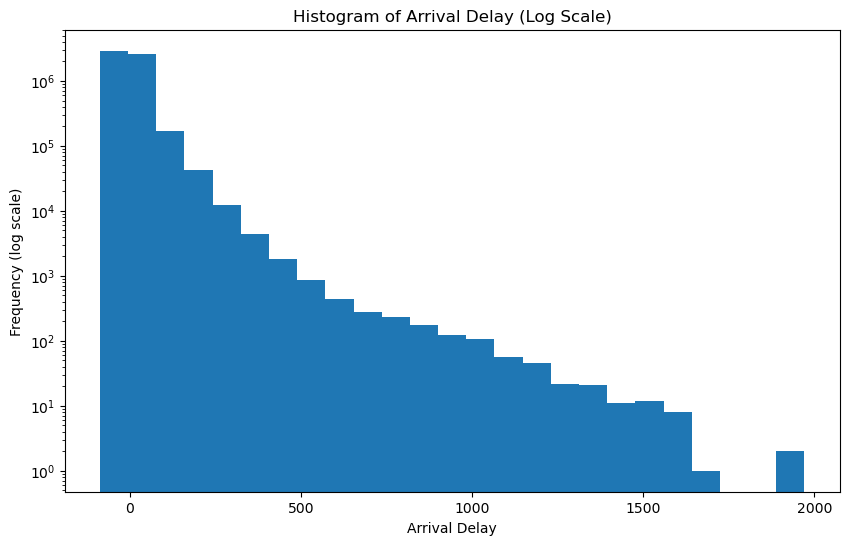
\includegraphics[width=0.6\textwidth]{../figures/arrivaldelay.png}
    \caption{Distribution of Arrival Delay in Minutes, plotted in logspace}
    \label{fig:arrivaldelay}
\end{figure}
 
As can be seen, the distribution of arrival delays is highly skewed, with a large number of flights arriving slightly early and slightly delayed, and a much smaller number of flights experiencing significant delays. Hence, we determine that our model should be robust to outliers.

Although we eventually determined that the various delay causes should not be included in the training of the final models, we still explored their correlation with the target variable. We can see that in Figure \ref{fig:delaycauses}, we see a sort of checkmark pattern indicating that the arrival delay is either highly correlated with airline delay, or completely uncorrelated. We note that we never see any data below \(y=x,\) since the arrival delay cannot be less than the departure delay.
\begin{figure}[h]
    \centering
    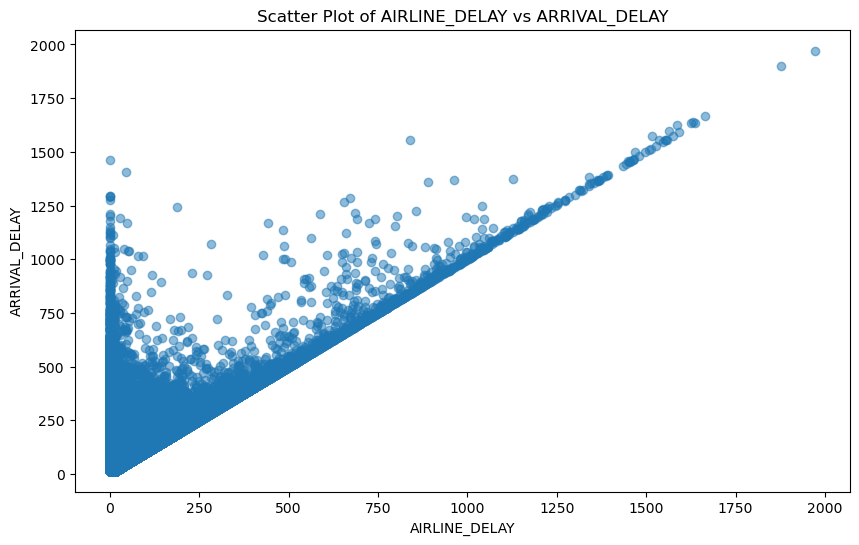
\includegraphics[width=0.6\textwidth]{../figures/arrivaldelayvsairlinedelay.png}
    \caption{Correlation of Arrival Delay with Departure Delay.}
    \label{fig:delaycauses}
\end{figure}

Finally, we explore the correlation of flight delays with different categorical features. For instance, we can view violin plots of arrival delays by airline, seen in Figure \ref{fig:arrivaldelaybyairline}. This plot displays the top 20 most frequent airlines in the dataset, with outliers removed for visibility. 
\begin{figure}[h]
    \centering
    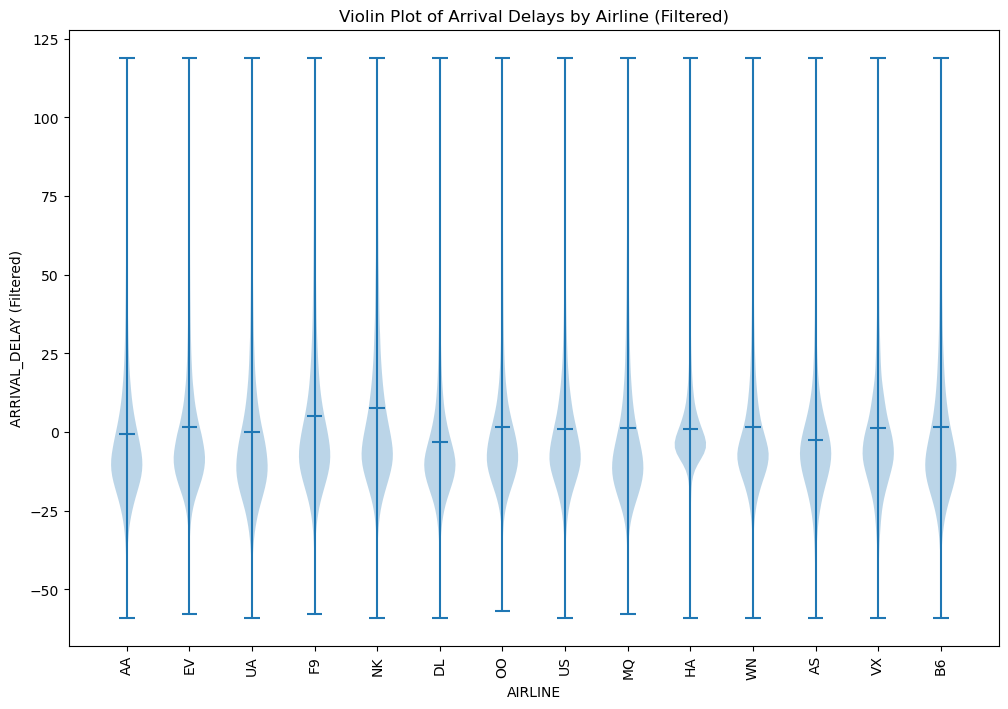
\includegraphics[width=0.6\textwidth]{../figures/arrivaldelaybyairlinefiltered.png}
    \caption{Arrival Delay by Airline, with outliers removed for visibility.}
    \label{fig:arrivaldelaybyairline}
\end{figure}

While these distributions appear similar, we calculate that the mean delay for each airline is statistically significantly different from the mean delay for other airlines, with a few exceptions. This suggests that there is a difference in the expected arrival delay for different airlines, which indicates that airline could be a useful feature in our model.
\section{Methods}
\subsection{Data Splitting}
Before splitting our data, we perform some preliminary data cleaning. First, we notice that some rows are missing values in the target variable, which we drop as they cannot be used for either training or testing, so are unusable. For missing values in other columns, we find that they exist only within a few columns. Five of these columns are delay cause columns, which is a lucky break as they are not available at prediction time so must be dropped anyways. The final column with missing values, cancellation reason, is actually missing all of its values, so we drop this value without hesitation, as it is similarly useless.

\begin{figure}[h]
    \centering
    \begin{tabular}{c|c}
        Column & Missing Values (\%) \\
        \hline
        \texttt{CANCELLATION\_REASON} & 100.00\% \\
        \texttt{AIR\_SYSTEM\_DELAY} & 81.39\% \\
        \texttt{SECURITY\_DELAY} & 81.39\% \\
        \texttt{AIRLINE\_DELAY} & 81.39\% \\
        \texttt{LATE\_AIRCRAFT\_DELAY} & 81.39\% \\
        \texttt{WEATHER\_DELAY} & 81.39\%
    \end{tabular}
    \caption{Percentage of missing values in columns with missing values.}
    \label{fig:missingvalues}
\end{figure}

As previously mentioned, our dataset consists of several categorical features, some continuous features, and some bounded continuous features (that are temporal in nature). It is important to note that these temporal features are not being used to predict future temporal values, but a different target variable entirely, which allows us to rule out the need for time-series analysis. We instead split our dataset into training, validation, and testing sets with a 60-20-20 random split. The dataset is over five million rows, and we consider this large enough that each set is representative of the overall dataset.
\subsection{Preprocessing}
To prepare our data for training, we perform several preprocessing steps. First, we determine whether any other features must be removed, because as the data was collected after the fact, some features might not be available at inference and would cause data leakage. We further find that the following columns must be removed: \texttt{WHEELS\_OFF}, \texttt{WHEELS\_ON}, \texttt{ARRIVAL\_TIME}, \texttt{TAXI\_IN}, \texttt{AIR\_TIME}, and \texttt{ELAPSED\_TIME}. 

\begin{figure}[h]
    \centering
    \begin{tabular}{c|c|c}
        Categorical & Continuous & Temporal \\ 
        \hline
        \texttt{AIRLINE} & \texttt{DEPARTURE\_DELAY} & \texttt{SCHEDULED\_DEPARTURE} \\ 
        \texttt{ORIGIN\_AIRPORT} & \texttt{TAXI\_OUT} & \texttt{DEPARTURE\_TIME} \\ 
        \texttt{DESTINATION\_AIRPORT} & \texttt{SCHEDULED\_TIME} & \texttt{SCHEDULED\_ARRIVAL} \\ 
        \texttt{DIVERTED} & \texttt{DISTANCE} \\ 
        \texttt{CANCELLED}
    \end{tabular}
    \caption{Training features and their type.}
    \label{fig:features}
\end{figure}

Among our categorical features (Figure \ref{fig:features}), we perform one-hot encoding on categorical features, use \texttt{StandardScaler} for continuous features, and use \texttt{MinMaxScaler} for temporal features, with one modification - the origin and destination airports have a very large number of unique values, so we keep the top 20 airports by frequency and aggregate all other airports into an "other" category to avoid high dimensionality. Finally, we fit the preprocessing pipeline on the training set and apply it to the validation and test sets.
\subsection{Model Training}
We train four different types of regression models: Elastic Net, Support Vector Regression (SVR) with Linear Kernel, Decision Tree, and XGBoost. Since the flight delay dataset consists of over five million rows, high-complexity models like random forest regressors or rbf kernel SVRs are simply infeasible to train. Therefore, we select simple models or those that scale relatively well. These above four will suffice.

For each model type, we perform hyperparameter tuning with grid-search over 1\% of the training data to train and 1\% of the training data to validate, then validate the best parameters for 4 random states on the whole validation set, select the best parameters, and then train the model with the best hyperparameters on the full training set. This allows us to efficiently search the hyperparameter space without excessive computational cost, while also still maintaining a representative sample of the data, as 1\% of five million rows is still \(\sim\)fifty thousand rows.
\subsubsection{Hyperparameter Tuning}
In Figure \ref{fig:hyperparameters}, we see the hyperparameters that were tested for each model type. There parameters were chosen for their breadth but also their representative nature of the search space, along with being few enough such that the hyperparameter search would be computationally inexpensive. For each combination of hyperparameters, we train and validate over our training data samples with four separate random state initializations, using root mean squared error (RMSE) as our evaluation metric, as we are in a regression setting and due to its penalization of larger errors and its maintenance of the same units as the target variable.
\begin{figure}[h]
    \centering
    \begin{small}
        \begin{tabular}{c|c|c|c}
            ElasticNet & SVR & Decision Tree & XGBoost \\
            \hline
            \texttt{alpha}: [.01, .1, 1, 10, 100] & \texttt{C}: [.1, 1, 10, 100] & \texttt{max\_depth}: [3, 7, 10] & \texttt{max\_depth}: [6, 9, 12] \\ 
            \texttt{l1\_ratio}: [0, .33, .67, 1] & \texttt{max\_iter}: [1000,10000] & & \texttt{subsample}: [.3, .5, .7, .9] \\
        \end{tabular}
    \end{small}
    \caption{Hyperparameter tested for each model type.}
    \label{fig:hyperparameters}
\end{figure}

After determining the best hyperparameters for each model type, the results of which can be found in Figure \ref{fig:hyperparametergrids}, we confirm their performance on the full validation set for four different random state initializations, ensuring that the selected hyperparameters generalize well. In fact, we never observed a case where the standard deviation of RMSE across random states was greater than 0.25 for any model type.
\begin{figure}
    \centering
    \begin{tabular}{c|c}
        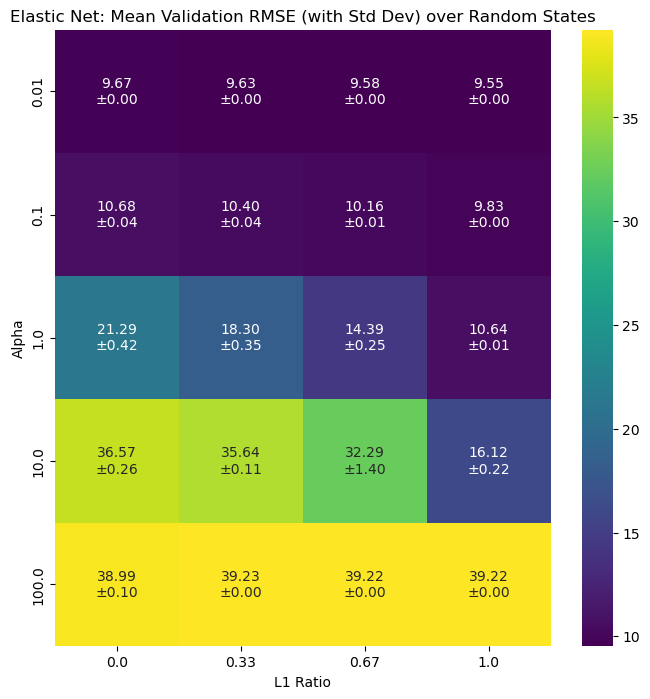
\includegraphics[width=0.45\textwidth]{../figures/elasticnethyperparam.png} & 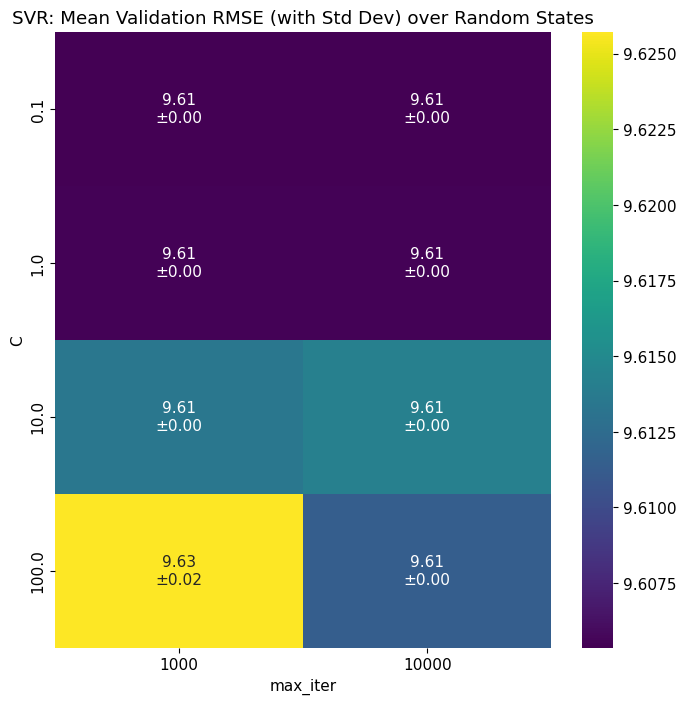
\includegraphics[width=0.45\textwidth]{../figures/svmhyperparam.png} \\
        \hline
        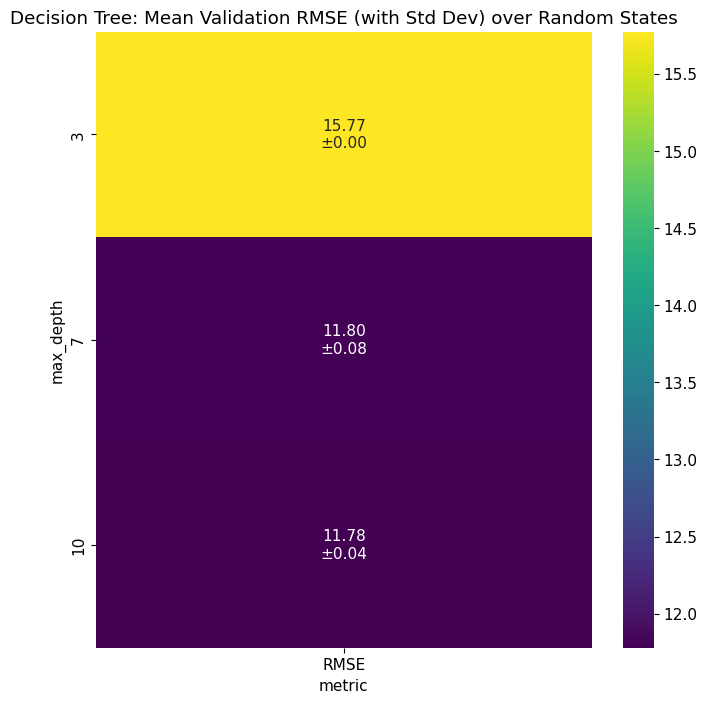
\includegraphics[width=0.45\textwidth]{../figures/decisiontreehyperparam.png} & 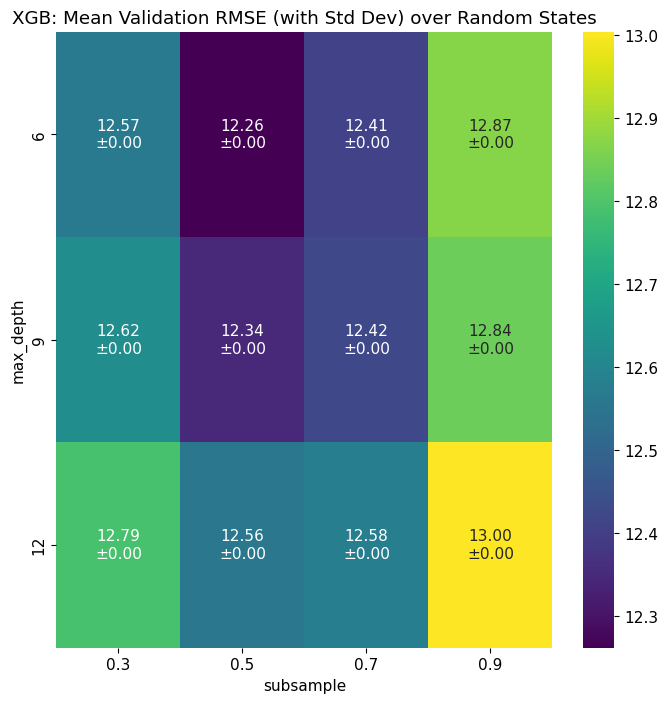
\includegraphics[width=0.45\textwidth]{../figures/xgboosthyperparam.png}
    \end{tabular}
    \caption{Mean validation RMSE with standard deviation across all hyperparameter combinations for each model. Note that darker colors correspond to lower loss.}
    \label{fig:hyperparametergrids}
\end{figure}
\subsubsection{Model Training}
Finally, we select the hyperparameters and random state initalization that provided the best RMSE on the validation set for each model type, and train the final models on the full training set.
\section{Results}
\subsection{Initial Analysis}
Evaluated against the test set, we find the following RMSE and \(R^2\) scores for each model type, as seen in Figure \ref{fig:testresults}, compared against the baseline model, which we selected to be the mean arrival delay in the training set for all flights.
\begin{figure}[h]
    \centering
    \begin{tabular}{c|c|c}
        Model & Test RMSE & Test \(R^2\) \\
        \hline
        Baseline & 39.2402 & 0.0000 \\
        Elastic Net & 9.5827 & 0.9404 \\
        SVR & 9.6204 & 0.9399 \\
        Decision Tree & 10.5147 & 0.9282 \\
        XGBoost & 9.4666 & 0.9418 \\
    \end{tabular}
    \caption{Test set results for all models compared to baseline. All models performed well, although we can see that XGBoost performed with the lowest RMSE and highest correlation.}
    \label{fig:testresults}
\end{figure}

We can also visualize a scatterplots to confirm these results, which may be viewed in Figure \ref{fig:scatterplots}. We notice that most predictions are quite accurate, with some undershooting earlier on in all models. Also notice that XGBoost gets a few of the extreme delays wrong, predicting them to be much lower than is actually the case, but this is for a handful of outliers. It is surprising that with these major outliers XGBoost still performs with the highest correlation/lowest RMSE, however it seems to get many more points more correct in the bottom left area, where the bulk of the data is located.
\begin{figure}
    \centering
    \begin{tabular}{c|c}
        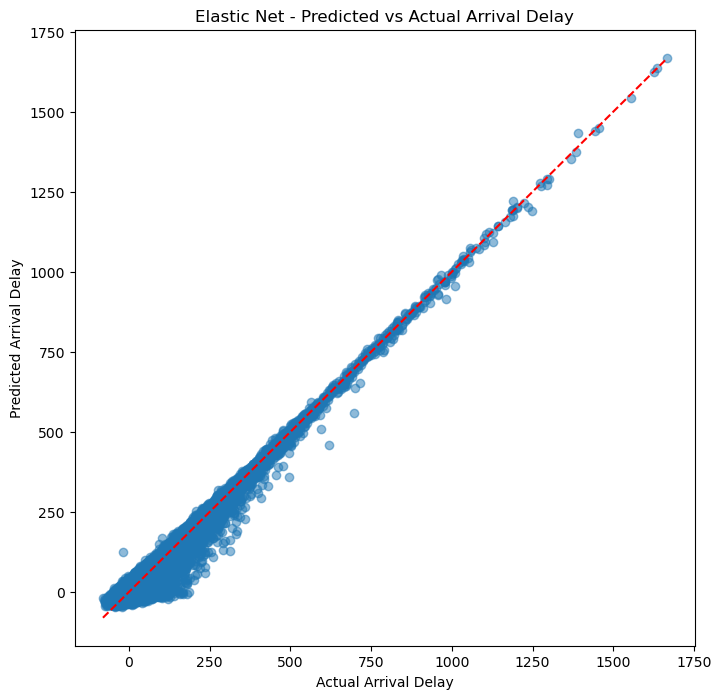
\includegraphics[width=0.45\textwidth]{../figures/elasticnetscatter.png} & 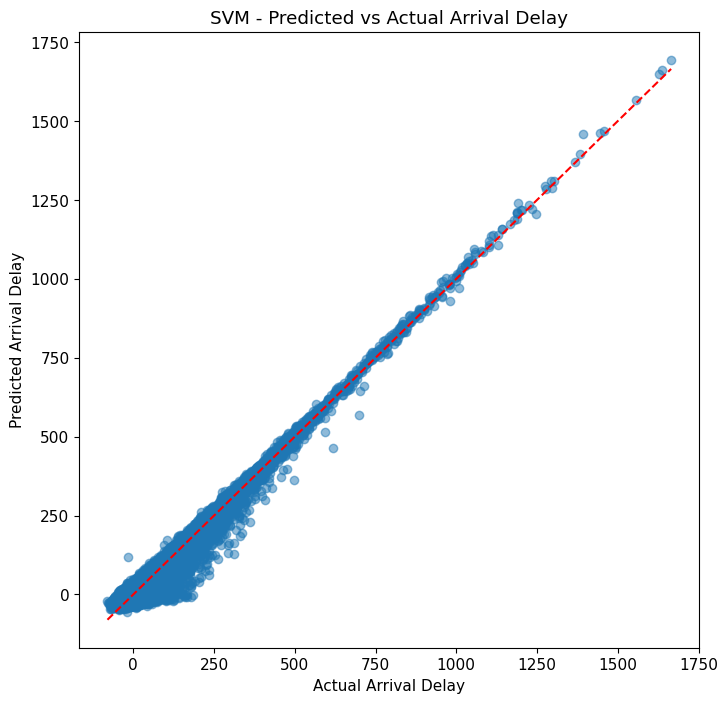
\includegraphics[width=0.45\textwidth]{../figures/svmscatter.png} \\
        \hline
        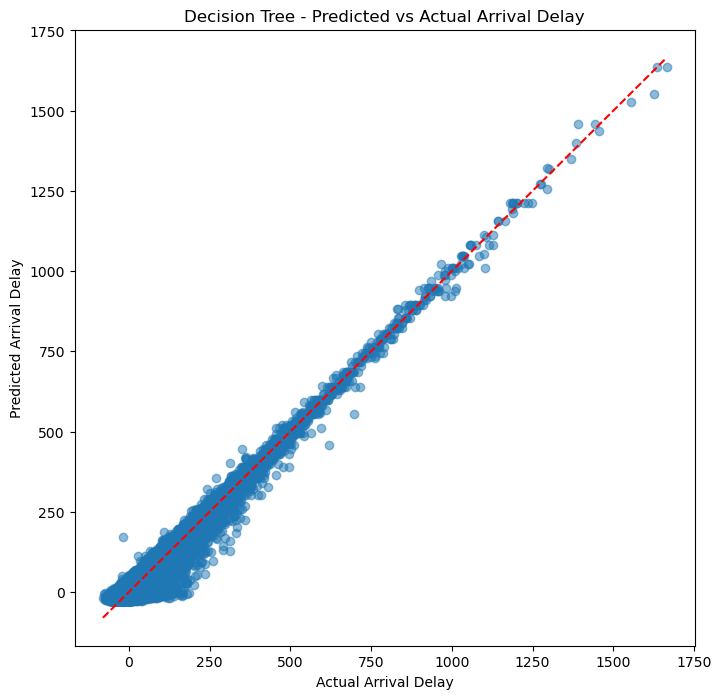
\includegraphics[width=0.45\textwidth]{../figures/decisiontreescatter.png} & 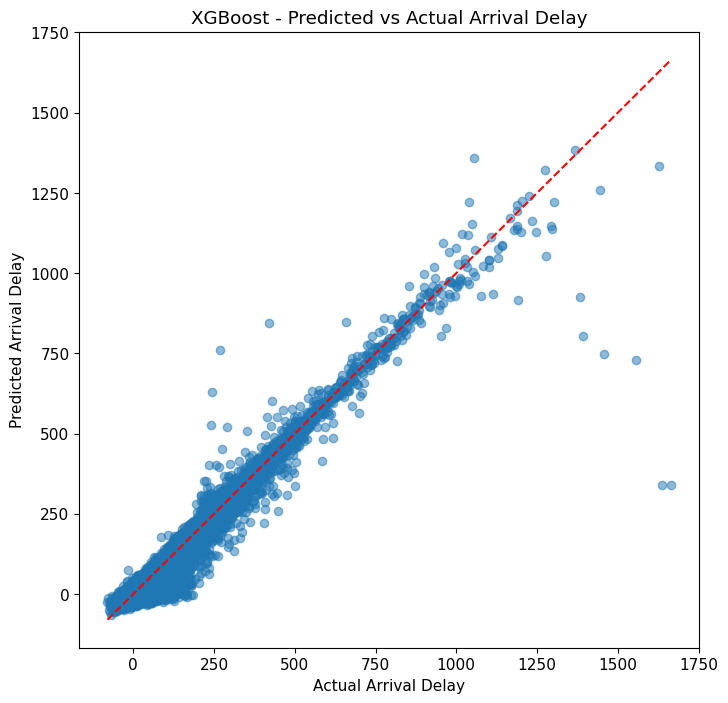
\includegraphics[width=0.45\textwidth]{../figures/xgboostscatter.png}
    \end{tabular}
    \caption{Scatter plots of predicted vs actual arrival delays for each model. The diagonal represents perfect predictions.}
    \label{fig:scatterplots}
\end{figure}
\newpage
\subsection{Interpretability}
\subsubsection{Global Interpretability}
\begin{figure}
    \centering
    \begin{tabular}{c|c}
        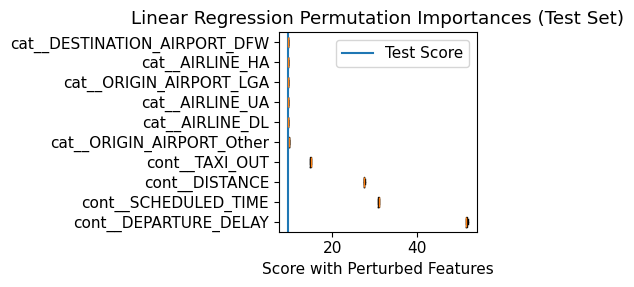
\includegraphics[width=0.45\textwidth]{../figures/elasticnetperturbation.png} & 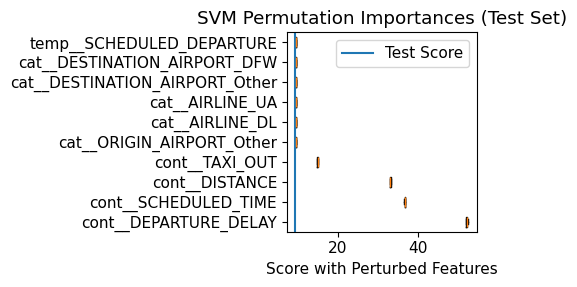
\includegraphics[width=0.45\textwidth]{../figures/svmperturbation.png} \\
        \hline
        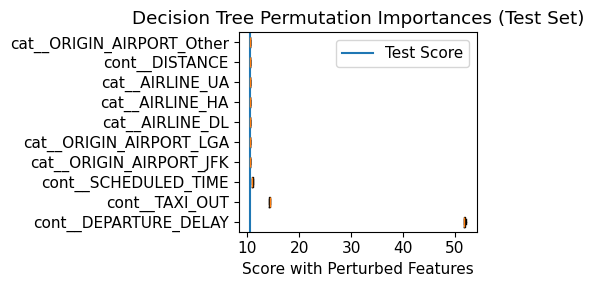
\includegraphics[width=0.45\textwidth]{../figures/decisiontreeperturbation.png} & 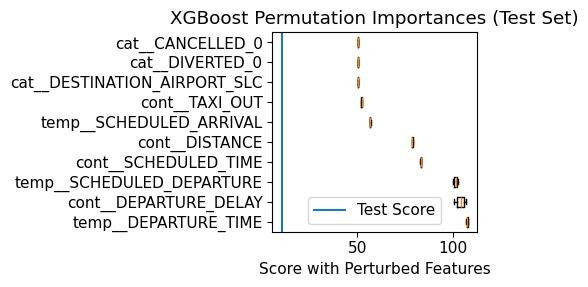
\includegraphics[width=0.45\textwidth]{../figures/xgboostperturbation.png}
    \end{tabular}
    \caption{Feature importance for each model type, determined via perturbation analysis.}
    \label{fig:featureimportance}
\end{figure}

We performed perturbation analysis on the final models to determine feature importance, as seen in Figure \ref{fig:featureimportance}. We find that across all models, the most important feature tends to be \texttt{DEPARTURE\_DELAY}, which makes sense as a delayed departure almost certainly results in a delayed arrival. Other important features include \texttt{TAXI\_OUT}, a feature that indicates the time taken to taxi from the gate to the runway, and \texttt{SCHEDULED\_DEPARTURE}, which indicates the time of day of departure. This makes sense, as flight volume is not uniform throughout the day, and so certain times of delay may be more prone to congestion and cascading delays. 

We see that elastic net and SVR have nearly identical feature importance rankings, but in particular, along with those mentioned above, that \texttt{DISTANCE} is also important, which makes sense as longer flights have more opportunity for delays to accumulate, especially due to weather conditions. Decision tree relies primarily on only a few metrics, which each successive ranking metric mattering less and less. XGBoost, on the other hand, seems to rely on a wider variety of features, including \texttt{DISTANCE}, \texttt{SCHEDULED\_ARRIVAL}, \texttt{CANCELLED}, \texttt{DIVERTED}, among others. This makes sense, as XGBoost is an ensemble of decision trees, and so is able to capture more complex relationships between features.

These results are unsurprising to us, as they align with our intuition about what features would be important in predicting flight delays. Overall, the models seem to be relying on reasonable features to make their predictions.
\subsubsection{Local Interpretability}
\begin{figure}
    \centering
    \begin{tabular}{c|c}
        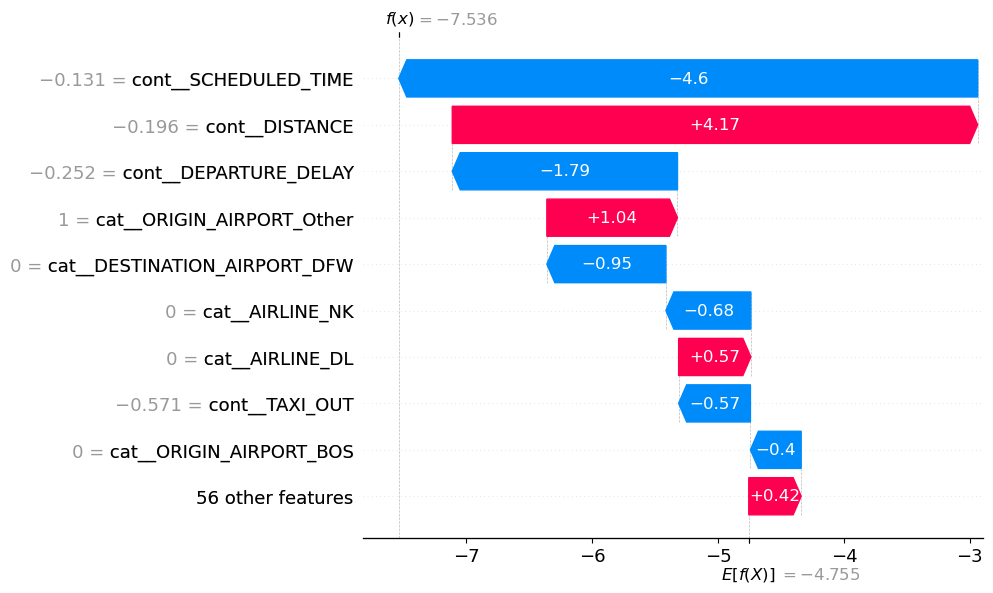
\includegraphics[width=0.45\textwidth]{../figures/elasticnetshap2.png} & 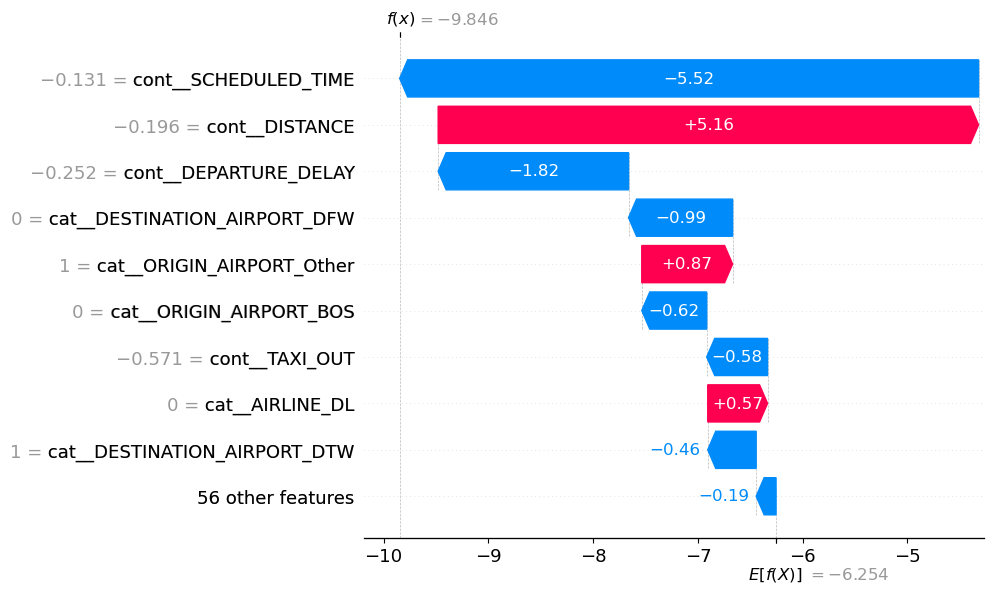
\includegraphics[width=0.45\textwidth]{../figures/svmshap2.png} \\
        \hline
        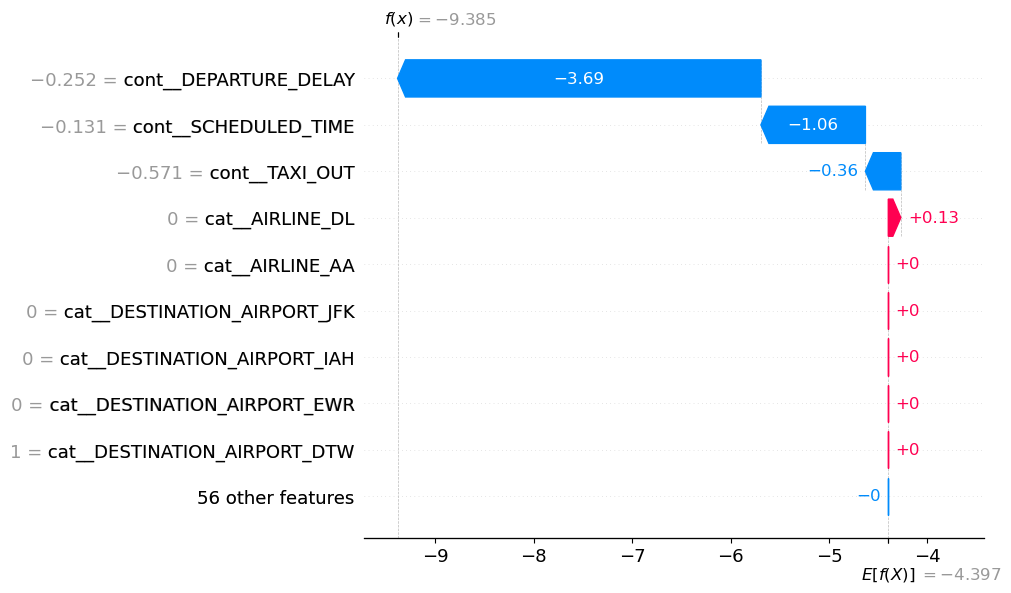
\includegraphics[width=0.45\textwidth]{../figures/decisiontreeshap2.png} & 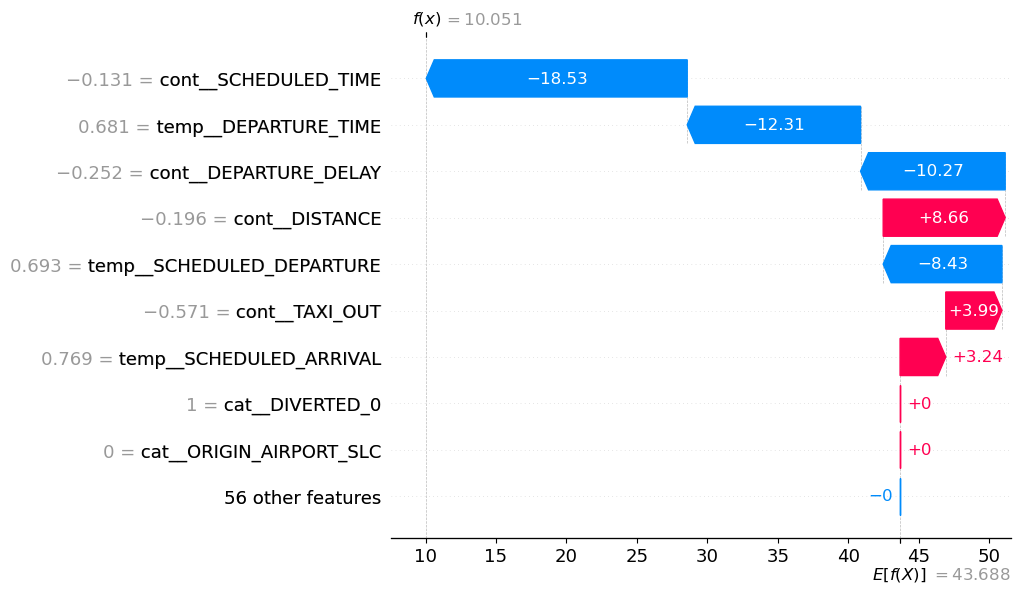
\includegraphics[width=0.45\textwidth]{../figures/xgboostshap2.png} \\
    \end{tabular}
    \caption{Shap values for each model across sample 2. Top-left: Elastic Net, Top-right: SVR, Bottom-left: Decision Tree, Bottom-right: XGBoost.}
    \label{fig:shap2}
\end{figure}
\begin{figure}
    \centering
    \begin{tabular}{c|c}
        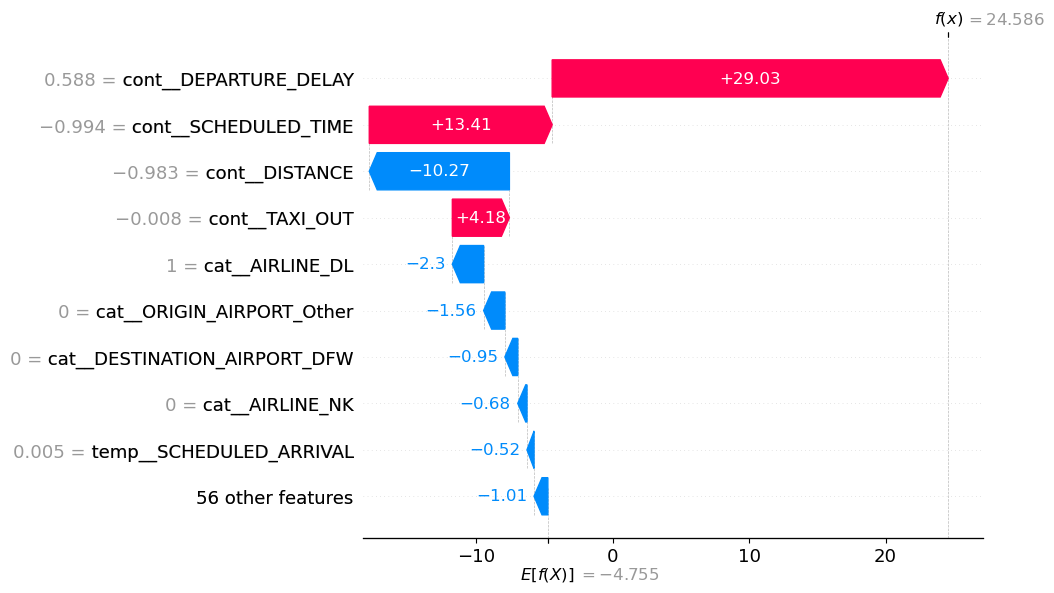
\includegraphics[width=0.45\textwidth]{../figures/elasticnetshap5.png} & 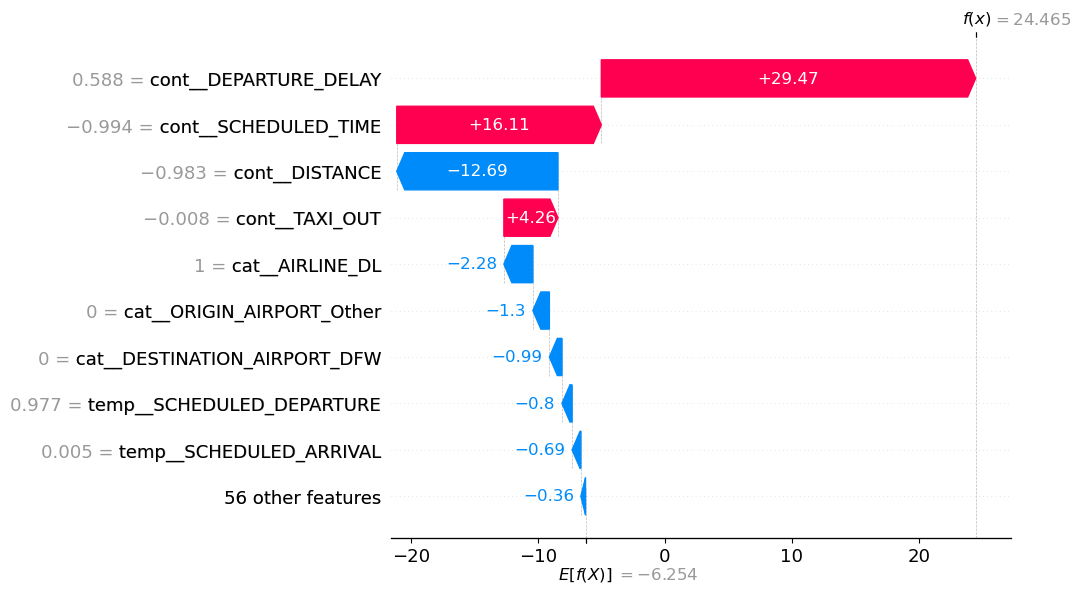
\includegraphics[width=0.45\textwidth]{../figures/svmshap5.png} \\
        \hline
        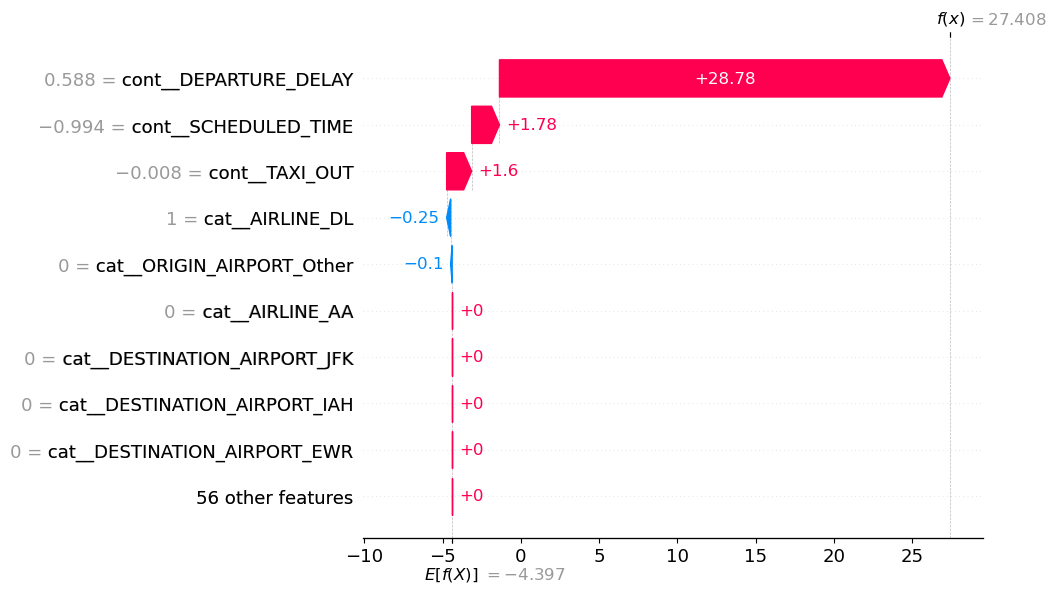
\includegraphics[width=0.45\textwidth]{../figures/decisiontreeshap5.png} & 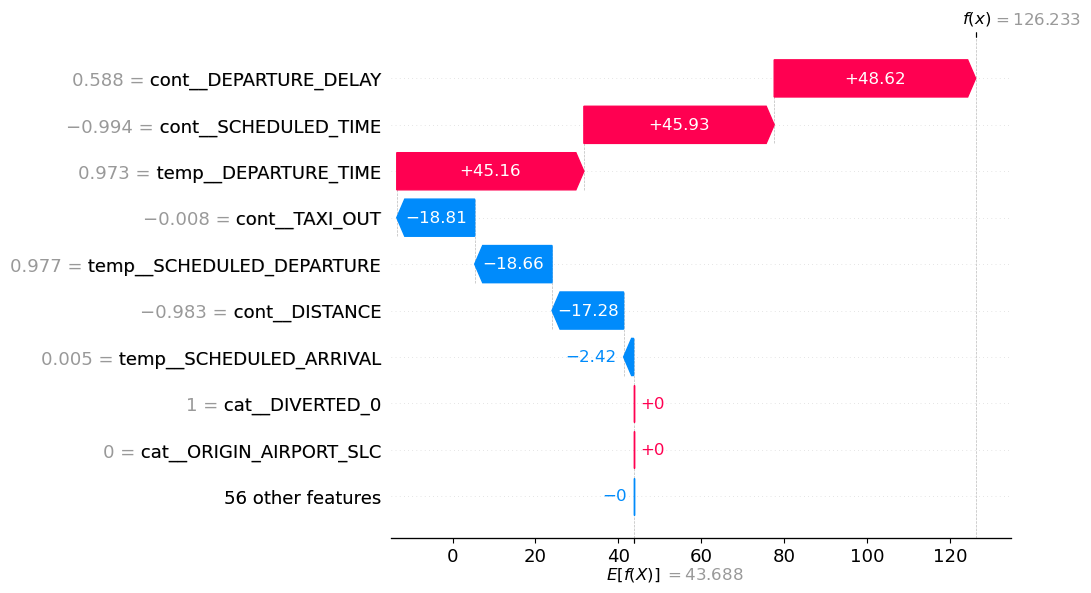
\includegraphics[width=0.45\textwidth]{../figures/xgboostshap5.png} \\
    \end{tabular}
    \caption{Shap values for each model across sample 5. Top-left: Elastic Net, Top-right: SVR, Bottom-left: Decision Tree, Bottom-right: XGBoost.}
    \label{fig:shap5}
\end{figure}
We also calculated SHAP values for five examples randomly selected from the test set. For consistency, we calculated SHAP values according to each model type for the same five examples. I have elected to display the waterfall plots for samples two (Figure \ref{fig:shap2}) and five (Figure \ref{fig:shap5}).
\newpage
From these plots, we can see much of our analysis from global feature importance is reflected here with respect to feature choice and number of features.
\section{Outlook}
While model performance is quite good, the large size of the dataset inhibited the selection of more complex models that may have outperformed those explored here. If more powerful computational resources were available, we may consider nonlinear kernels for support vector regression, as well as random forest regression. With the same resources, we also may consider global SHAP value calculation, which would provide more robust feature importance rankings.

With respect to outlier delays, we might consider training a separate model to predict outlier conditions, and then separate models on typical conditions and outlier conditions, as the prior should be fine-grained for day-to-day use, while the other may be helpful for resource allocation during extreme disruptive events.
\bibliographystyle{plain}
\bibliography{refs}
\end{document}